\documentclass[12pt]{article}

\usepackage{a4wide} % уменьшает поля
\usepackage[utf8]{inputenc}
\usepackage[russian]{babel} % включает русский язык
\usepackage{graphicx} % позволяет подключить .eps - файлы
\usepackage{amsmath}
\usepackage{amsthm} % теоремы от AMS
\usepackage{amssymb} % для работы с математическими R и проч.
\usepackage{floatrow}
\usepackage{mathrsfs}
\usepackage[section]{placeins}
\usepackage{indentfirst} % абзац после заголовка
\usepackage{misccorr} % точки в заголовках

%\graphicspath{{pics/}}


%\newtheoremstyle{rusdef}
%  {3pt}% measure of space to leave above the theorem. E.g.: 3pt
%  {3pt}% measure of space to leave below the theorem. E.g.: 3pt
%  {\itshape}% name of font to use in the body of the theorem
%  {\parindent}% measure of space to indent
%  {\bfseries}% name of head font
%  {.}%
%  {.5em}%
%  {}
   
  
\theoremstyle{rusdef}
\renewcommand\qedsymbol{$\blacksquare$}
\newtheorem{remark}{Замечание}
\newtheorem{theorem}{Теорема}
\newtheorem{definition}{Определение}
\newtheorem{proposition}{Утверждение}

\newcommand*{\hm}[1]{#1\nobreak\discretionary{}{\hbox{$\mathsurround=0pt #1$}}{}}
\newcommand{\scalar}[2]{\left<#1,#2\right>}
\newcommand{\const}{\ensuremath{\operatorname{const}}}
\newcommand{\sgn}{\ensuremath{\operatorname{sgn}}}
\renewcommand{\d}[1]{\ensuremath{\operatorname{d}\!{#1}}}
\newcommand\abs[1]{\left\lvert #1 \right\rvert} % модуль
\newcommand\brackets[1]{\left( #1 \right)} % скобки
\newcommand{\R}{\ensuremath{\mathbb{R}}} % R - мн-во вещественных чисел
\newcommand{\N}{\ensuremath{\mathbb{N}}} % N - мн-во натуральных чисел
\newcommand{\Z}{\ensuremath{\mathbb{Z}}} % Z - мн-во целых чисел
\renewcommand{\C}{\ensuremath{\mathbb{C}}} % C - мн-во комплексных чисел
\newcommand{\E}{\ensuremath{\mathcal{E}}} % E --- эллипсоид
\newcommand{\norm}[1]{\left\lVert #1 \right\rVert} % норма
\DeclareMathOperator*{\thus}{\Rightarrow} % следствие с возможностью использовать limits
\DeclareMathOperator*{\tolim}{\to} % стремление с возможностью использовать limits
\DeclareMathOperator*{\Argmax}{Argmax} % Argmax с возмножностью использовать limits
\DeclareMathOperator{\rank}{rank} % ранг
\DeclareMathOperator{\e}{e} % экспонента

\newcommand{\rpm}{\sbox0{$1$}\sbox2{$\scriptstyle\pm$}
\raise\dimexpr(\ht1)/2\relax\box2 } % крутой плюс-минус

\begin{document}
\thispagestyle{empty}

\begin{center}
\ \vspace{-3cm}


\includegraphics[width=0.5\textwidth]{msu.eps}\\

{\scshape Московский Государственный Университет имени М.~В.~Ломоносова}\\
Факультет Вычислительной Математики и Кибернетики\\
Кафедра Системного Анализа
\vfill

{\LARGE Лабораторная работа по курсу <<Математические модели в экономике>>}

{\LARGE Оценка влияния государственной энергетической политики на потенциал экономического роста в России}
\vspace{.5cm}

\end{center}

\vspace{1cm}

\begin{flushright}
\large
\textit{Студент 415 группы}\\
В.~С.~Терёшин\\
\vspace{5mm}
\textit{Руководитель практики}\\
к.ф.-м.н., ассистент А.В.Рудева

\end{flushright}

\vfill

\begin{center}
{\large
Москва, 2014г.}
\end{center}

\newpage
\tableofcontents
\newpage
\section{Постановка задачи}
\begin{enumerate}
\item Построить и проанализировать зависимости от доли экспорта в выпуске нефтегазовой отрасли следующих макроэкономических показателей:
\begin{enumerate}
\item темп роста цен,
\item темп роста производства,
\item параметр неэффективности,
\item доля налогов в добавленной стоимости электроэнергетики,
\item доля зарплаты и распределяемой прибилы в добавленной стоимости НГК,
\item доля потребления населения к ВВП,
\item доля государственных расходов к ВВП,
\item доля добавленной стоимости 1-го сектора в ВВП,
\item доля добавленной стоимости 2-го сектора в ВВП,
\item доля добавленной стоимости 3-го сектора в ВВП,
\item отношение инвестиций во 2-ой сектор к выпуску 2-го сектора,
\item отношение инвестиций в 3-ий сектор к выпуску 3-го сектора.
\end{enumerate}
Объяснить результат
\item
Объяснить влияние параметра неэффективности на макроэкономические показатели. Для этого провести сравнение результатов по двум вариантам модели: с учетом неэффективности производства в энергопотребляющем секторе и без учета неэффективности.
\end{enumerate}

\section{Анализ зависимостей и сравнение моделей}
Ниже приведены графики соответствующих зависимостей. Графики для первой модели, не учитывающей неэффективность производства в энергопотребляющем секторе, приведены красным, для второй модели, учитывающей неэффективность, они изображены синим. Рассмотрим вторую модель. Из рис. 1 видно, что с ростом доли экспорта продукции НГК темп инфляции увеличивается. Это объясняется увеличением темпа прироста денежной массы в государстве (увеличение экспорта влечёт увеличение финансовых поступлений в НГК и в государство в виде налогов). В связи с увеличением темпа инфляции при неизменной структуре производственной системы темп роста производства падает при изменении
доли экспорта с $w_3 = 0.25$ до $w_3 = 0.34$, что видно из рис. 2. Затем темп роста производства начинает расти. Это объясняется тем, что в производственной системе начинаются перестройки. Увеличение объёма экспорта предприятий НГК ведёт к потребности увеличения производственных фондов, однако фондообразующим сектором является «неэффективный» первый сектор. В результате, увеличивается потребление продукции первого сектора при неизменном объёме производства. Это влечёт к увеличению эффективности функционирования первого сектора, что видно из рис. 3 на промежутке $w_3 \in [0.25, 0.4]$. При $w_3 > 0.4$ наблюдается резкий рост эффективности производства первого сектора, задержки в реализации товаров существенно уменьшаются и для адекватного описания производства в первом секторе может использоваться первая модель (модель Хаутеккера-Иохансена). При $w_3 > 0.34$ начинает возрастать доля добавочной стоимости первого сектора и уменьшаться доля добавочной стоимости второго сектора в ВВП, что видно из рис. 8 и рис. 9. Это объясняется более быстрым ростом добавочной стоимости первого сектора по отношению ко второму с ростом потребности в его продукции со стороны НГК и государства, объём
потребления которого также возрастает в связи с увеличением финансовых поступлений. Из рис. 7 видно, что отношение государственных расходов к ВВП растёт при увеличении $w_3$ от $0.25$ до $0.39$. Затем это отношение уменьшается в связи с увеличением числа инвестиций в первый и третий сектора, в которых расширяется
производство. В этой связи уменьшается и доля потребления населения в ВВП, что видно из рис. 6. На рис. 11 и рис. 12 отражено существенное увеличение числа инвестиций во второй и третий сектора при $w_3 > 0.36$, возникающее с потребностьюв расширении производства в НГК. Из рисунков видно, что первая модель неадек-
ватно описывает имеющуюся ситуацию, в случае неэффективно функционирующего первого производственного сектора. Пусть теперь первый сектор экономики функционирует эффективно (задержек в реализации продукции нет). Тогда все получающиеся графики оказываются монотонными. С ростом доли экспорта продукции НГК растёт темп инфляции (за счёт
увеличения денежной массы в государстве), падает темп производства (за счёт увеличения темпа инфляции и отсутствия существенных перестроек в производственной системе). Перераспределения долей производства в секторах не происходит, всё большую долю в ВВП начинают занимать добавочные стоимости второго и третьего секторов (продукция второй отрасли требуется для производства в третьей), доля первого сектора падает. С увеличением инвестиций во все сектора и увеличением государственных расходов (с связи с увеличем финансовых поступлений от экспорта) уменьшается потребление населения. Анализ влияния увеличения доли экспорта продукции НГК в первой и второй моделях показывает, что в двух этих моделях экономика развивается по существенно разным сценариям. Таким образом, пренебречь влиянием неэффективности функционирования первого сектора нельзя и следует использовать вторую модель. Однако некоторые показатели (темп инфляции, доля добавочной стоимости третьего сектора
в ВВП) ведут себя в этих моделях качественно одинаково и при их анализе можноиспользовать более простую модель Хаутеккера-Иохансена.
\begin{figure}[h!]
	\centering
	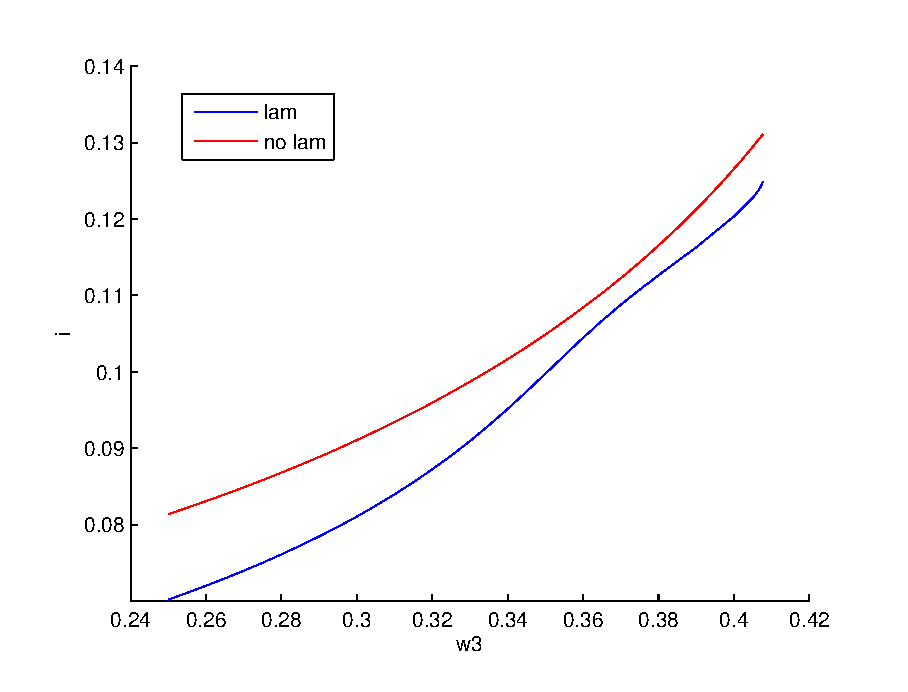
\includegraphics[scale=0.8]{pics/w3_i.eps}
	\caption{Темп роста цен в зависимости от доли экспорта в НГК.}
\end{figure}
\begin{figure}[h!]
	\centering
	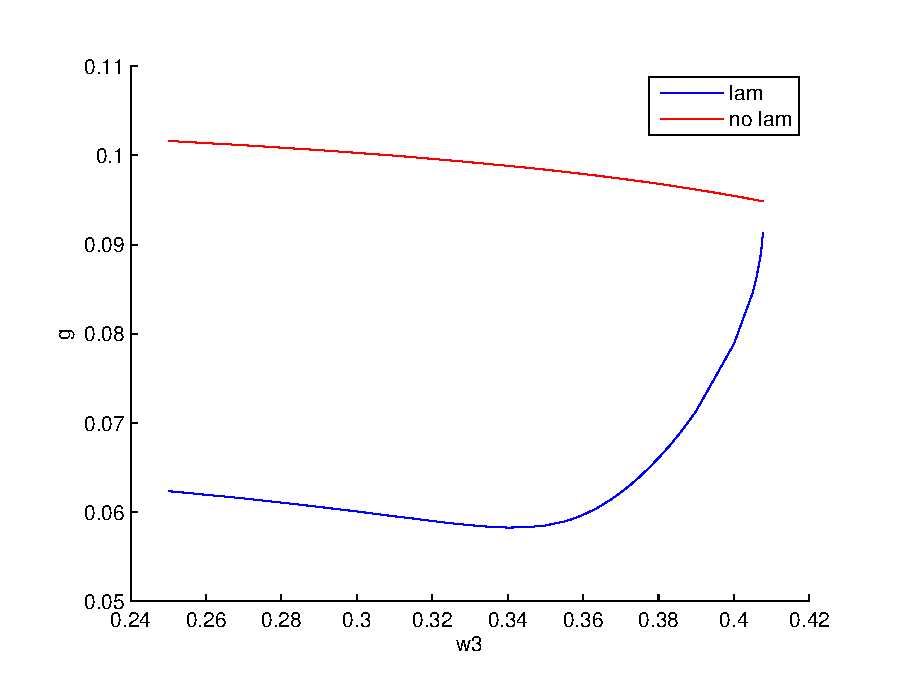
\includegraphics[scale=0.8]{pics/w3_g.eps}
	\caption{Темп роста производства в зависимости от доли экспорта в НГК.}
\end{figure}
\begin{figure}[h!]
	\centering
	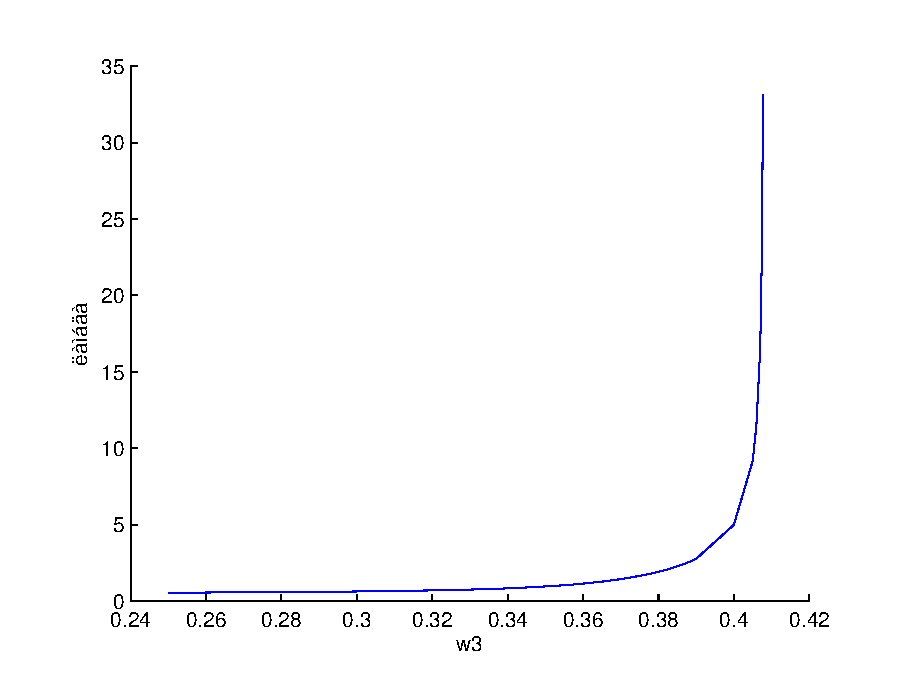
\includegraphics[scale=0.8]{pics/w3_lambda.eps}
	\caption{Параметр неэффективности в зависимости от доли экспорта в НГК.}
\end{figure}
\begin{figure}[h!]
	\centering
	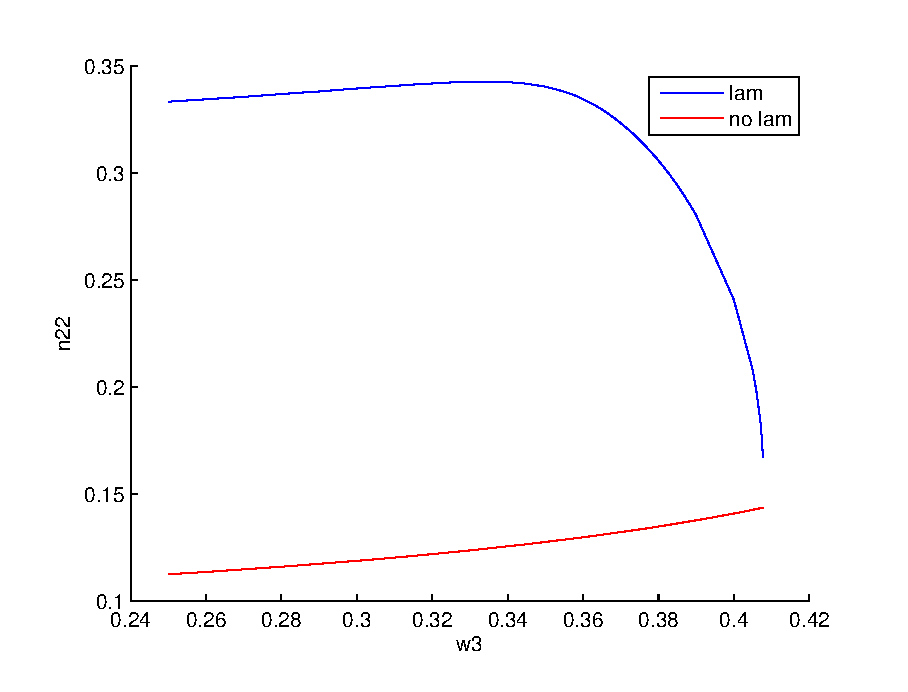
\includegraphics[scale=0.8]{pics/w3_n22.eps}
	\caption{доля налогов в добавленной стоимости электроэнергетики в зависимости от доли экспорта в НГК.}
\end{figure}
\begin{figure}[h!]
	\centering
	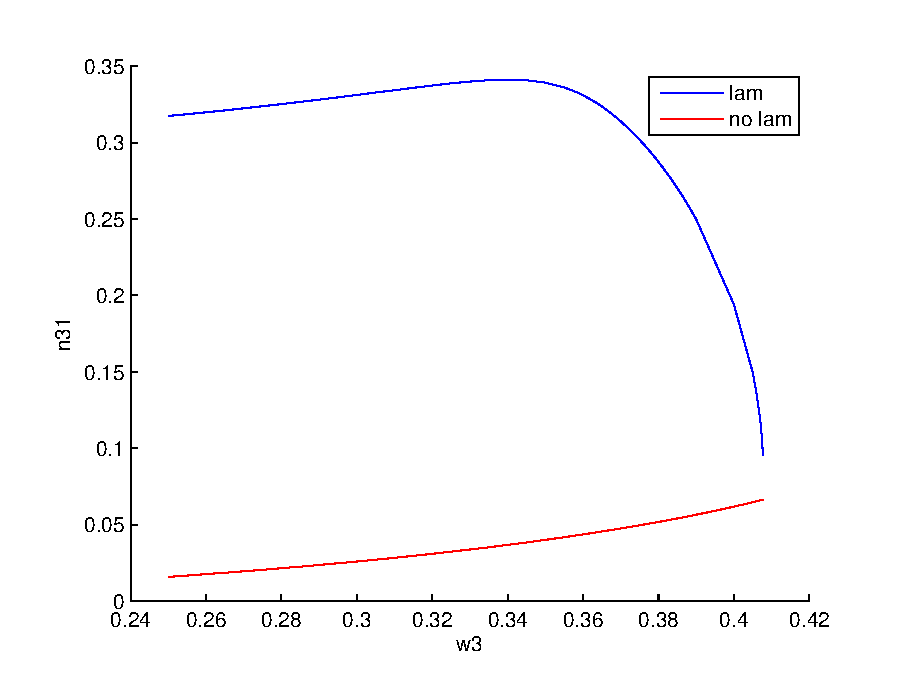
\includegraphics[scale=0.8]{pics/w3_n31.eps}
	\caption{Доля зарплаты и распределяемой прибыли в добавленной стоимости НГК в зависимости от доли экспорта в НГК.}
\end{figure}
\begin{figure}[h!]
	\centering
	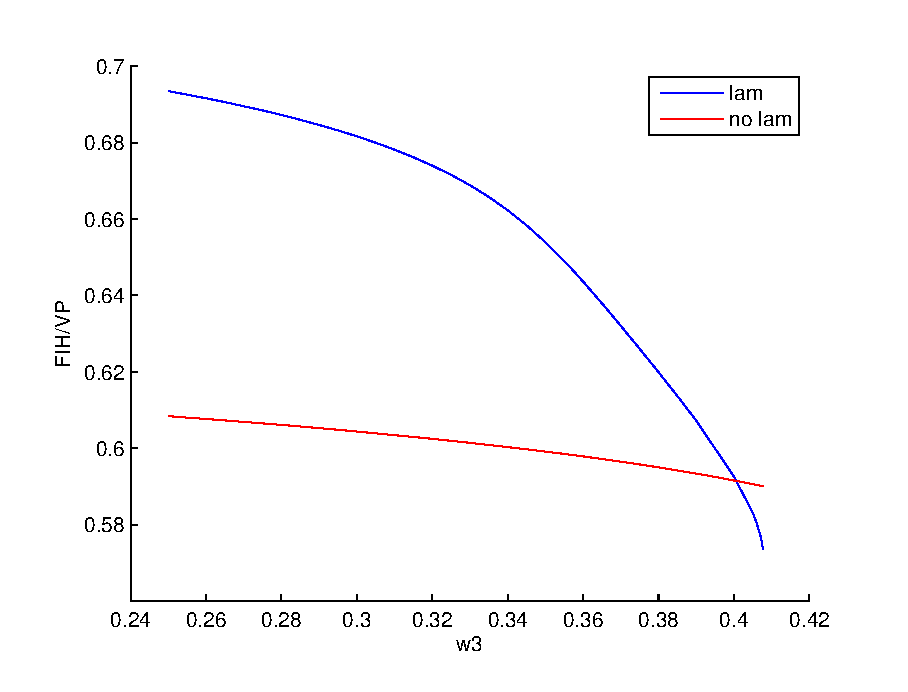
\includegraphics[scale=0.8]{pics/w3_FIH-VP.eps}
	\caption{отношение потребления населения к ВВП в зависимости от доли экспорта в
	НГК.}
\end{figure}
\begin{figure}[h!]
	\centering
	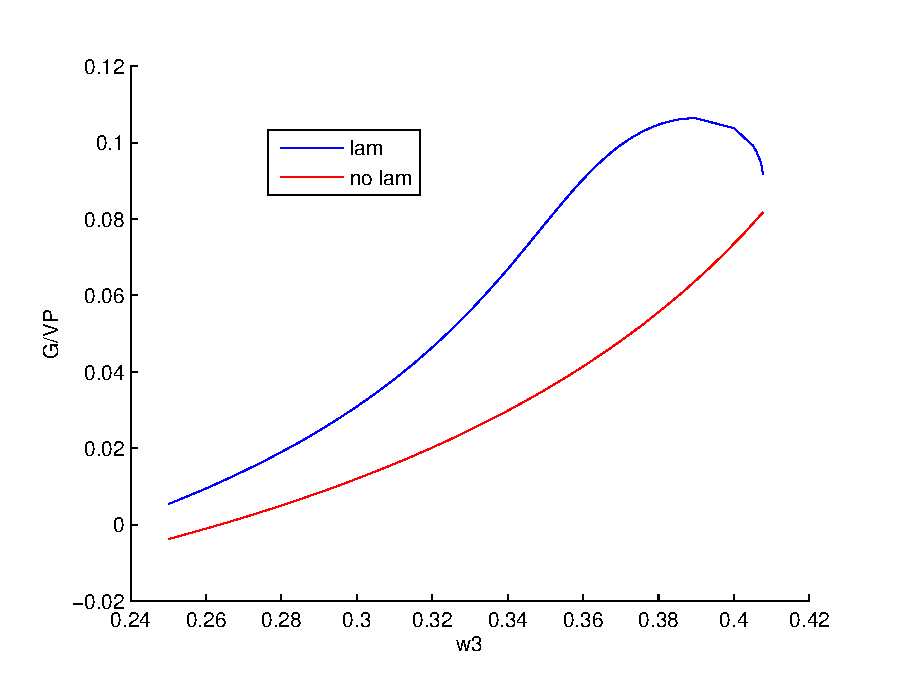
\includegraphics[scale=0.8]{pics/w3_G-VP.eps}
	\caption{отношение государственных расходов к ВВП в зависимости от доли экспорта
		в НГК.}
\end{figure}
\begin{figure}[h!]
	\centering
	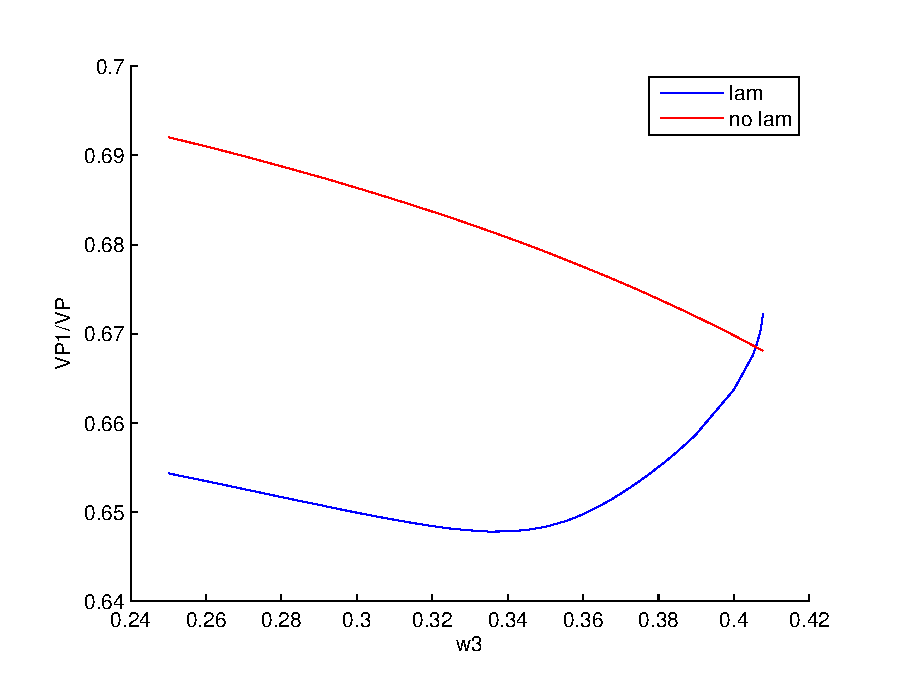
\includegraphics[scale=0.8]{pics/w3_VP1-VP.eps}
	\caption{доля добавленной стоимости 1-го сектора в ВВП в зависимости от доли
		экспорта в НГК.}
\end{figure}
\begin{figure}[h!]
	\centering
	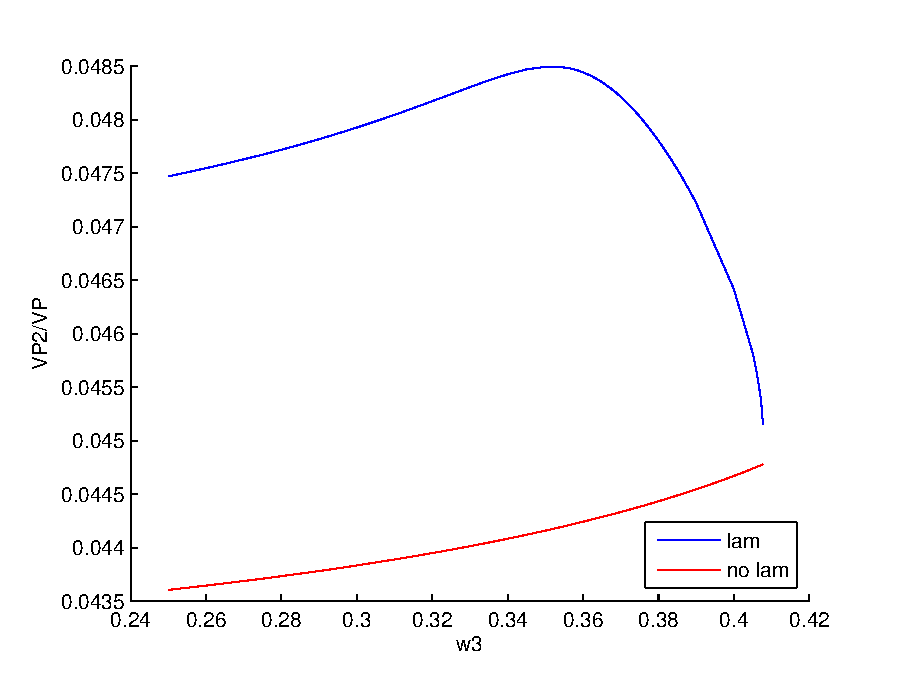
\includegraphics[scale=0.8]{pics/w3_VP2-VP.eps}
	\caption{доля добавленной стоимости 2-го сектора в ВВП в зависимости от доли
		экспорта в НГК.}
\end{figure}
\begin{figure}[h!]
	\centering
	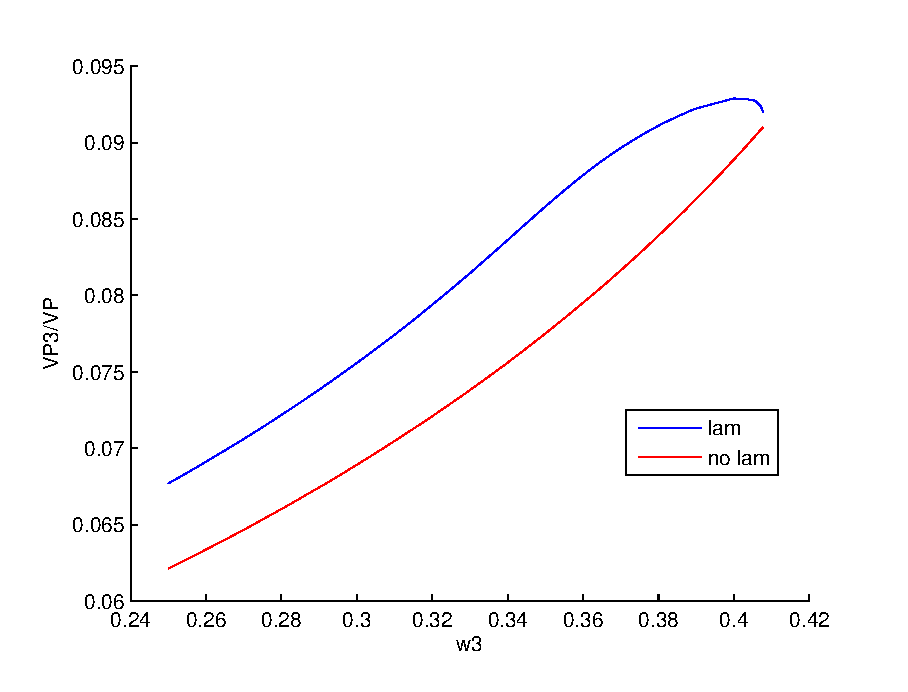
\includegraphics[scale=0.8]{pics/w3_VP3-VP.eps}
	\caption{доля добавленной стоимости 3-го сектора в ВВП в зависимости от доли
		экспорта в НГК.}
\end{figure}
\begin{figure}[h!]
	\centering
	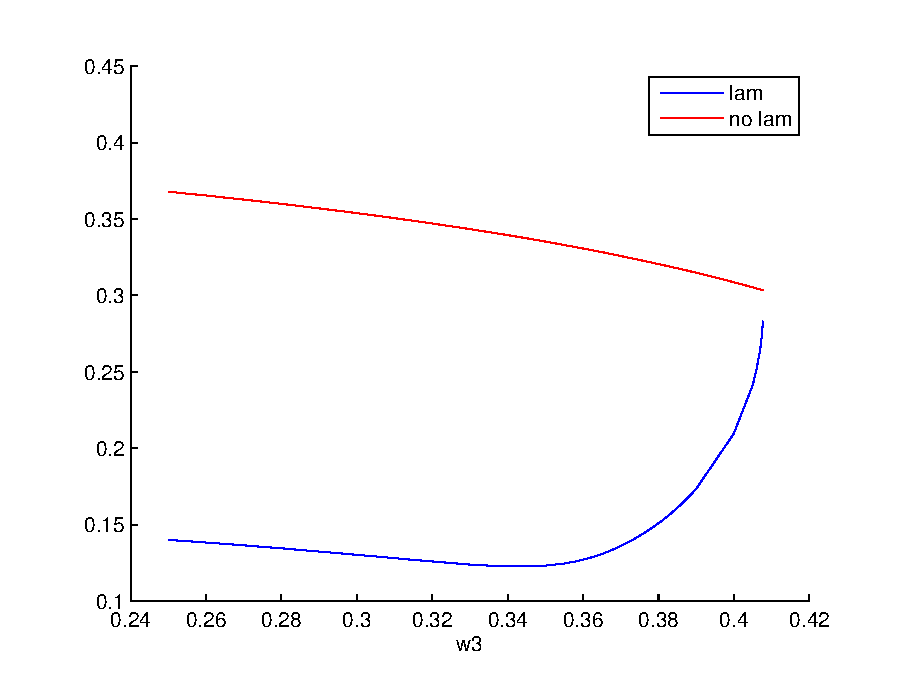
\includegraphics[scale=0.8]{pics/w3_unknown2.eps}
	\caption{отношение инвестиций во 2-ой сектор к выпуску 2-го сектора в зависимости от доли экспорта в НГК.}
\end{figure}
\begin{figure}[h!]
	\centering
	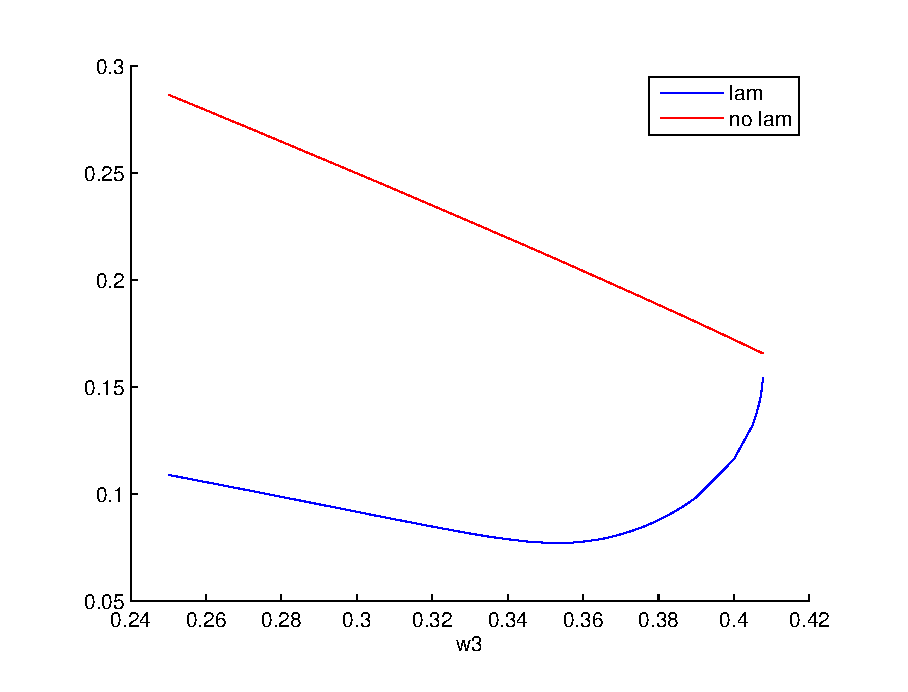
\includegraphics[scale=0.8]{pics/w3_unknown3.eps}
	\caption{отношение инвестиций во 3-ой сектор к выпуску 3-го сектора в зависимости от доли экспорта в НГК.}
\end{figure}\newpage
\begin{thebibliography}{99}
        \bibitem{example} Example.
\end{thebibliography}
\end{document}